\documentclass[UTF8]{ctexart}

\title{电子技术基础实验第八周实验报告}

\author{王磊\quad2022012972}

\date{\today}

\usepackage{geometry}
\geometry{a4paper,scale=0.8}

\usepackage{graphicx}
\usepackage{subfigure}
\usepackage{float}

\usepackage{amsmath}

\usepackage{listings}
\usepackage{xcolor}
\usepackage{framed}
\lstdefinestyle{verilogStyle}{
    language=verilog,
    basicstyle=\ttfamily,
    keywordstyle=\color{blue},
    commentstyle=\color{green},
    stringstyle=\color{red},
    numbers=left,
    numberstyle=\tiny\color{gray},
    breaklines=true,
    showstringspaces=false,
    columns = fixed,
    basewidth = 0.5em,
    captionpos=b,
}
\newcommand{\subsubsubsection}[1]{\paragraph{#1}\mbox{}\\}
\setcounter{secnumdepth}{4} % how many sectioning levels to assign numbers to
\setcounter{tocdepth}{4} % how many sectioning levels to show in ToC
%设置段落间距
\setlength{\parskip}{0.5em}
%令小标题左对齐
\CTEXsetup[format={\Large\bfseries}]{section}
%首行不缩进
\setlength{\parindent}{0pt}
\begin{document}
\maketitle
%小标题
\section{task1\_2\&task1\_3}
由于task1\_2是task1\_3的子模块,因此不单独介绍task1\_2。task1\_2要求的移位显示可以通过下类代码实现;
\begin{framed}
    \begin{lstlisting}[language=verilog,style=verilogStyle]
        first_num <= {first_num[7:0],input_temp[3:0]};
    \end{lstlisting}
\end{framed}
\subsection{模块设计}
数码管显示模块、分频模块与week6一致,不再赘述。
\subsubsection{矩阵按键模块}
\subsubsubsection{代码实现}
\begin{framed}
    \begin{lstlisting}[language=verilog,style=verilogStyle]
always @(posedge clk or posedge rst) begin
    if(rst) begin
        state <= 2'b00; 
		hl <= 4'b1111;
    end
    else begin
        case (state)
            2'b00: begin
				hl <= 4'b1110;
                state <= 2'b01;
            end
            2'b01: begin
				hl <= 4'b1101;
                state <= 2'b10;
            end
            2'b10: begin
				hl <= 4'b1011;
                state <= 2'b11;
            end
            2'b11: begin
				hl <= 4'b0111;
                state <= 2'b00;
            end
            default: begin
				hl <= 4'b1111;
                state <= 2'b00;
            end
        endcase
    end
end 
assign hl_vl = {hl,vl};  
    \end{lstlisting}
\end{framed}
在这个模块中,通过控制hl的输出使能矩阵键盘的不同列,实现了矩阵键盘的扫描,并将结果输出到hl\_vl中。
\subsubsubsection{仿真结果}
\begin{figure}[H]
    \centering
    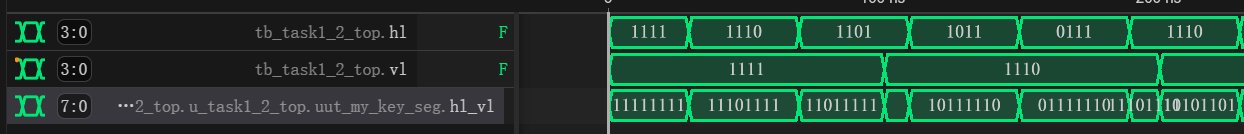
\includegraphics[width=0.8\textwidth]{task1_3_1.png}
    \caption{矩阵键盘仿真结果}
\end{figure}
\subsubsection{按键处理模块}
\subsubsubsection{代码实现}
\begin{framed}
    \begin{lstlisting}[language=verilog,style=verilogStyle]
//process the origin input to a simple one
reg [2:0] input_type;
parameter NUMBER = 3'b001;
parameter OPERATOR = 3'b010;
parameter EQUAL = 3'b100;

reg [4:0] input_temp;

always @ (posedge clk,posedge rst) begin
	if (rst) begin
		input_type <= 3'b000;
		input_temp <= 5'b00000;
	end
	else begin
		case (hl_vl)
			8'b0111_0111: begin
				//for =  
				input_type <= EQUAL;
				input_temp <= 5'b00000;   
			end
			8'b1011_0111: begin
				//for and   
				input_type <= OPERATOR;
				input_temp <= AND_OPERATOR;
			end
			8'b1101_0111: begin
				//for 0
				input_type <= NUMBER;
				input_temp <= 5'b00000;
			end
			8'b1110_0111: begin
				//for or     
				input_type <= OPERATOR;
				input_temp <= OR_OPERATOR;
			end
			8'b0111_1011: begin
				//for +     
				input_type <= OPERATOR;
				input_temp <= ADD_OPERATOR;
			end
			8'b1011_1011: begin
				//for 3
				input_type <= NUMBER;
				input_temp <= 5'b00011;
			end
			8'b1101_1011: begin
				//for 2
				input_type <= NUMBER;
				input_temp <= 5'b00010;
			end
			8'b1110_1011: begin
				//for 1
				input_type <= NUMBER;
				input_temp <= 5'b00001;
			end
			8'b0111_1101: begin      
				//for -     
				input_type <= OPERATOR;
				input_temp <= SUB_OPERATOR;
			end
			8'b1011_1101: begin
				//for 6
				input_type <= NUMBER;
				input_temp <= 5'b00110;
			end
			8'b1101_1101: begin
				//for 5
				input_type <= NUMBER;
				input_temp <= 5'b00101;
			end
			8'b1110_1101: begin
				//for 4
				input_type <= NUMBER;
				input_temp <= 5'b00100;
			end
			8'b0111_1110: begin      
				//for compare
				input_type <= OPERATOR;
				input_temp <= COMPARE_OPERATOR;
			end
			8'b1011_1110: begin
				//for 9
				input_type <= NUMBER;
				input_temp <= 5'b01001;
			end
			8'b1101_1110: begin
				//for 8
				input_type <= NUMBER;
				input_temp <= 5'b01000;
			end
			8'b1110_1110: begin
				//for 7
				input_type <= NUMBER;
				input_temp <= 5'b00111;
			end
			default: begin
				input_type <= 3'b000;
				input_temp <= 5'b00000;
			end
		endcase
	end
end
    \end{lstlisting}
\end{framed}
在这个模块中,根据hl\_vl的输入,将其转换为对应的操作数或操作符,并将其输出到input\_type和input\_temp中。
\subsubsubsection{仿真结果}
\begin{figure}[H]
    \centering
    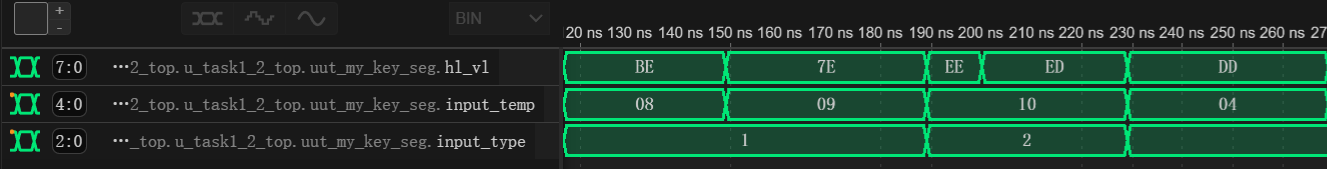
\includegraphics[width=0.8\textwidth]{task1_3_2.png}
    \caption{按键处理模块仿真结果}
\end{figure}
\subsubsection{状态机模块}
为了实现计算器的功能,我实现了一个简单的mearly状态机,其状态转移图如下:
\begin{figure}[H]
    \centering
    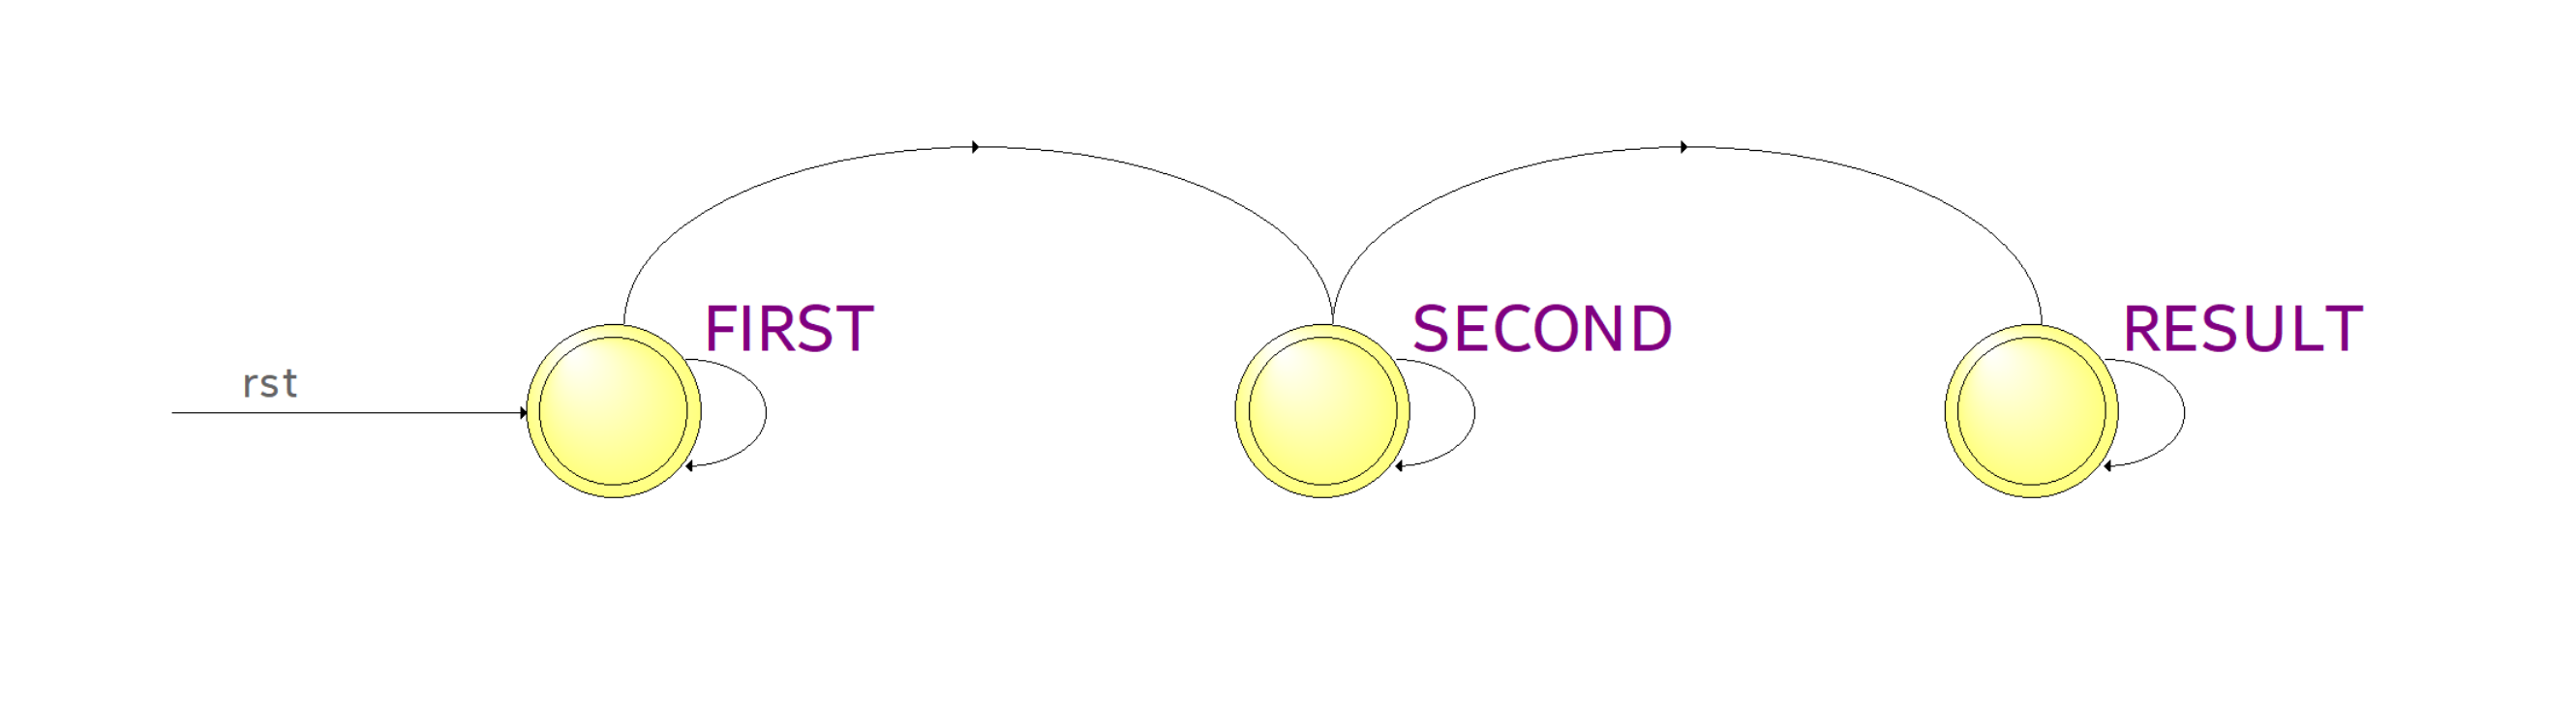
\includegraphics[width=0.8\textwidth]{task1_3_3.png}
    \caption{状态机状态转移图}
\end{figure}
其中,\texttt{FIRST}为显示第一个操作数,\texttt{SECOND}为显示第二个操作数,\texttt{RESULT}为显示计算结果。
\subsubsubsection{代码实现}
\begin{framed}
    \begin{lstlisting}[language=verilog,style=verilogStyle]
//try to use mealy machine to solve the problem
reg [2:0] FSM_state;
parameter FIRST = 3'b001;
parameter SECOND = 3'b010;
parameter RESULT = 3'b100;
reg [4:0] operator;
parameter OR_OPERATOR = 5'b00001;
parameter AND_OPERATOR = 5'b00010;
parameter ADD_OPERATOR = 5'b00100;
parameter SUB_OPERATOR = 5'b01000;
parameter COMPARE_OPERATOR = 5'b10000;

//the first part of the FSM, trying to get state according to input
reg [11:0] first_num;
reg [11:0] second_num;
reg [15:0] result;
always @(posedge clk, posedge rst) begin
	if(rst) begin
		FSM_state <= FIRST;
		operator <= 5'b00000;
		first_num <= 12'b0000_0000_0000;
		second_num <= 12'b0000_0000_0000;
	end
	else begin
		case(FSM_state)
			FIRST: begin
				if(input_type == NUMBER) begin
					first_num <= {first_num[7:0],input_temp[3:0]};
					FSM_state <= FIRST;
				end
				else if(input_type == OPERATOR) begin
					operator <= input_temp;
					FSM_state <= SECOND;
				end
				else begin
					FSM_state <= FIRST;
				end
			end
			SECOND: begin
				if(input_type == NUMBER) begin
					second_num <= {second_num[7:0],input_temp[3:0]};
					FSM_state <= SECOND;
				end
				else if(input_type == EQUAL) begin
					FSM_state <= RESULT;
				end
				else begin
					FSM_state <= SECOND;
				end
			end
			RESULT: begin
				case(operator)
					OR_OPERATOR: begin
						result <= first_num | second_num;
						FSM_state <= RESULT;
					end
					AND_OPERATOR: begin
						result <= first_num & second_num;
						FSM_state <= RESULT;
					end
					ADD_OPERATOR: begin
						result[3:0] <= (first_num[3:0] + second_num[3:0])%10;
						result[7:4] <= (first_num[7:4] + second_num[7:4] + (first_num[3:0] + second_num[3:0])/10)%10;
						result[11:8] <= (first_num[11:8] + second_num[11:8] + (first_num[7:4] + second_num[7:4] + (first_num[3:0] + second_num[3:0])/10)/10)%10;
						result[15:12] <= (first_num[11:8] + second_num[11:8] + (first_num[7:4] + second_num[7:4] + (first_num[3:0] + second_num[3:0])/10)/10)/10;
						FSM_state <= RESULT;
					end
					SUB_OPERATOR: begin
						result[3:0] <= (first_num[3:0] - second_num[3:0])%10;
						result[7:4] <= (first_num[7:4] - second_num[7:4] + (first_num[3:0] - second_num[3:0])/10)%10;
						result[11:8] <= (first_num[11:8] - second_num[11:8] + (first_num[7:4] - second_num[7:4] + (first_num[3:0] - second_num[3:0])/10)/10)%10;
						result[15:12] <= (first_num[11:8] - second_num[11:8] + (first_num[7:4] - second_num[7:4] + (first_num[3:0] - second_num[3:0])/10)/10)/10;
						FSM_state <= RESULT;
					end
					COMPARE_OPERATOR: begin
						if(first_num > second_num) begin
							result <= 12'b1;
						end
						else begin
							result <= 12'b0;
						end
						FSM_state <= RESULT;
					end
					default: begin
						result <= 12'b0;
						FSM_state <= RESULT;
					end
				endcase
			end
			default: begin
				FSM_state <= FIRST;
			end
	endcase
	end
end
    \end{lstlisting}
\end{framed}
以上为mearly状态机的第一部分,作用为根据输入切换状态,同时计算结果。
\begin{framed}
    \begin{lstlisting}[language=verilog,style=verilogStyle]
//the second part of the FSM, trying to show the result according to the state
always @(posedge clk, posedge rst) begin
	if(rst) begin
		data <= 16'b0000_0000_0000_0000;
	end
	else begin
		case(FSM_state)
			FIRST: begin
				data <= first_num;
			end
			SECOND: begin
				data <= second_num;
			end
			RESULT: begin
				data <= result;
			end
			default: begin
				data <= 16'b0000_0000_0000_0000;
			end
		endcase
	end
end
    \end{lstlisting}
\end{framed}
mearly状态机的第二部分,作用为根据状态显示对应的结果。
\subsubsubsection{仿真结果}
\begin{figure}[H]
    \centering
    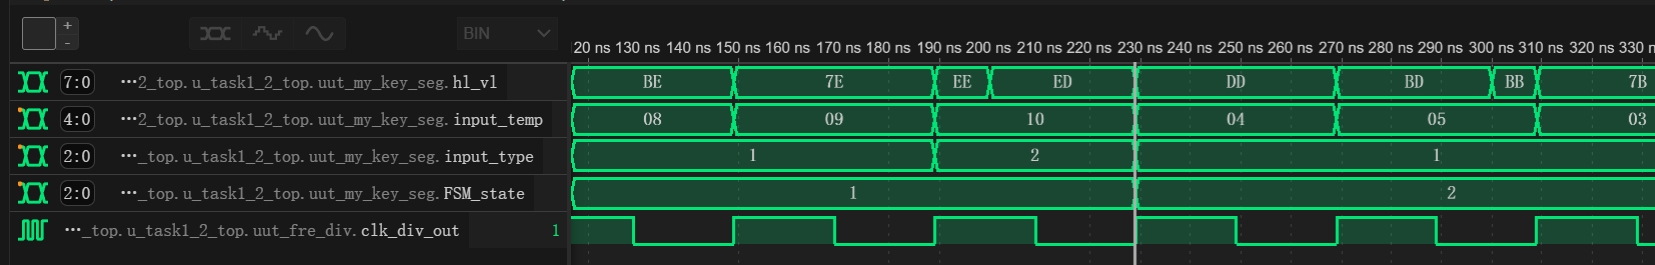
\includegraphics[width=0.8\textwidth]{task1_3_4.png}
    \caption{状态机模块仿真结果1}
\end{figure}
由上图可以看出,当\texttt{input\_type}为1时,\texttt{FSM\_state}会维持在\texttt{FIRST}状态。而当\texttt{input\_type}为2时,\texttt{FSM\_state}会转移到\texttt{SECOND}状态。证明状态机切换正常。
\begin{figure}[H]
    \centering
    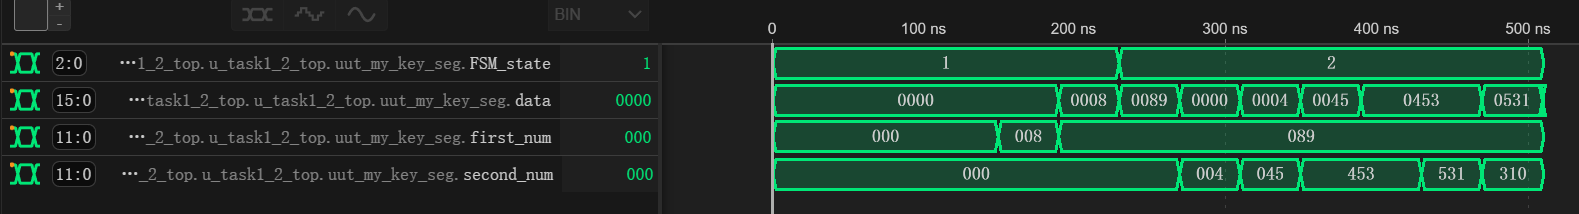
\includegraphics[width=0.8\textwidth]{task1_3_5.png}
    \caption{状态机模块仿真结果2}
\end{figure}
由上图可以看出,当\texttt{FSM\_state}为\texttt{FIRST}状态时,\texttt{data}与\texttt{first\_num}保持一致,而当\texttt{FSM\_state}为\texttt{SECOND}状态时,\texttt{data}与\texttt{second\_num}保持一致。证明状态机显示正常。
\subsection{仿真设计}
仿真结果已在上文中给出,代码实现如下。
\subsubsection{代码实现}
\begin{framed}
    \begin{lstlisting}[language=verilog,style=verilogStyle]
//~ `New testbench
`timescale 1ns/1ps
`include "task1_2_top.v"

module tb_task1_2_top;

    // task1_2_top Parameters
    parameter PERIOD = 10;

    // task1_2_top Inputs
    reg [3:0] vl = 0;
    reg clk = 0;
    reg rst = 0;

    // task1_2_top Outputs
    wire [3:0] hl;
    wire [3:0] digit;
    wire [7:0] seg;

    task1_2_top u_task1_2_top (
        .clk(clk),
        .rst(rst),
        .vl(vl[3:0]),
        .hl(hl[3:0]),
        .digit(digit[3:0]),
        .seg(seg[7:0])
    );

    initial begin
        $dumpfile(".\\wave\\tb_task1_2_top.vcd");
        $dumpvars(0, tb_task1_2_top);
        clk = 0;
        rst = 0;
        vl = 4'b1111;
        rst = 1;
        #10
        rst = 0;
        #500
        $finish;
    end

    always begin
        #1 clk = ~clk;
    end

    always begin
        #100
        vl = 4'b1110;
        #100
        vl = 4'b1101;
        #100
        vl = 4'b1011;
        #100
        vl = 4'b0111;
    end

endmodule
    \end{lstlisting}
\end{framed}
\section{task2\_2}
\subsection{模块设计}
分频模块、数码管显示模块与week6一致,不再赘述。
\subsubsection{地址生成模块}
\subsubsubsection{代码实现}
\begin{framed}
    \begin{lstlisting}[language=verilog,style=verilogStyle]
module addrgen(
    input clk,
    input rst,
    output reg [7:0] addr
);

always @(posedge clk or posedge rst) begin
    if(rst) begin
        addr <= 8'b00000000;
    end
    else begin
        addr <= addr + 1;
    end
end
endmodule
    \end{lstlisting}
\end{framed}
作用为每1s将addr加1。
\subsubsubsection{仿真结果}
\begin{figure}[H]
    \centering
    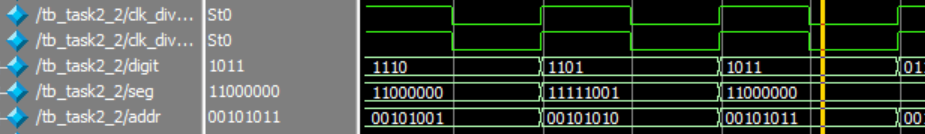
\includegraphics[width=0.8\textwidth]{task2_2_1}
    \caption{地址生成模块仿真结果}
\end{figure}

\end{document}